%%%%%%%%%%%%%%%%%%%%%%%%%%%%%%%%%%%%%%%%%
% Wenneker Article
% LaTeX Template
% Version 2.0 (28/2/17)
%
% This template was downloaded from:
% http://www.LaTeXTemplates.com
%
% Authors:
% Vel (vel@LaTeXTemplates.com)
% Frits Wenneker
%
% License:
% CC BY-NC-SA 3.0 (http://creativecommons.org/licenses/by-nc-sa/3.0/)
%
%%%%%%%%%%%%%%%%%%%%%%%%%%%%%%%%%%%%%%%%%

%----------------------------------------------------------------------------------------
%	PACKAGES AND OTHER DOCUMENT CONFIGURATIONS
%----------------------------------------------------------------------------------------

\documentclass[10pt, letter, twocolumn]{article} % 10pt font size (11 and 12 also possible), A4 paper (letterpaper for US letter) and two column layout (remove for one column)

%%%%%%%%%%%%%%%%%%%%%%%%%%%%%%%%%%%%%%%%%
% Wenneker Article
% Structure Specification File
% Version 1.0 (28/2/17)
%
% This file originates from:
% http://www.LaTeXTemplates.com
%
% Authors:
% Frits Wenneker
% Vel (vel@LaTeXTemplates.com)
%
% License:
% CC BY-NC-SA 3.0 (http://creativecommons.org/licenses/by-nc-sa/3.0/)
%
%%%%%%%%%%%%%%%%%%%%%%%%%%%%%%%%%%%%%%%%%

%----------------------------------------------------------------------------------------
%	PACKAGES AND OTHER DOCUMENT CONFIGURATIONS
%----------------------------------------------------------------------------------------

\usepackage[english]{babel} % English language hyphenation

\usepackage{microtype} % Better typography

\usepackage{amsmath,amsfonts,amsthm} % Math packages for equations

\usepackage[svgnames]{xcolor} % Enabling colors by their 'svgnames'

\usepackage[hang, small, labelfont=bf, up, textfont=it]{caption} % Custom captions under/above tables and figures

\usepackage{subcaption}

\usepackage{booktabs} % Horizontal rules in tables

\usepackage{lastpage} % Used to determine the number of pages in the document (for "Page X of Total")

\usepackage{multirow}

\usepackage{xfrac}

\usepackage{graphicx} % Required for adding images

\usepackage{enumitem} % Required for customising lists
\setlist{noitemsep} % Remove spacing between bullet/numbered list elements

\usepackage{sectsty} % Enables custom section titles
\allsectionsfont{\usefont{OT1}{phv}{b}{n}} % Change the font of all section commands (Helvetica)

%----------------------------------------------------------------------------------------
%	MARGINS AND SPACING
%----------------------------------------------------------------------------------------

\usepackage{geometry} % Required for adjusting page dimensions

\geometry{
	top=1cm, % Top margin
	bottom=1.5cm, % Bottom margin
	left=2cm, % Left margin
	right=2cm, % Right margin
	includehead, % Include space for a header
	includefoot, % Include space for a footer
	%showframe, % Uncomment to show how the type block is set on the page
}

\setlength{\columnsep}{7mm} % Column separation width

%----------------------------------------------------------------------------------------
%	FONTS
%----------------------------------------------------------------------------------------

\usepackage[T1]{fontenc} % Output font encoding for international characters
\usepackage[utf8]{inputenc} % Required for inputting international characters

\usepackage{XCharter} % Use the XCharter font

%----------------------------------------------------------------------------------------
%	HEADERS AND FOOTERS
%----------------------------------------------------------------------------------------

\usepackage{fancyhdr} % Needed to define custom headers/footers
\pagestyle{fancy} % Enables the custom headers/footers

\renewcommand{\headrulewidth}{0.0pt} % No header rule
\renewcommand{\footrulewidth}{0.4pt} % Thin footer rule

\renewcommand{\sectionmark}[1]{\markboth{#1}{}} % Removes the section number from the header when \leftmark is used

%\nouppercase\leftmark % Add this to one of the lines below if you want a section title in the header/footer

% Headers
\lhead{} % Left header
\chead{\textit{\thetitle}} % Center header - currently printing the article title
\rhead{} % Right header

% Footers
\lfoot{} % Left footer
\cfoot{} % Center footer
\rfoot{\footnotesize Page \thepage\ of \pageref{LastPage}} % Right footer, "Page 1 of 2"

\fancypagestyle{firstpage}{ % Page style for the first page with the title
	\fancyhf{}
	\renewcommand{\footrulewidth}{0pt} % Suppress footer rule
}

%----------------------------------------------------------------------------------------
%	TITLE SECTION
%----------------------------------------------------------------------------------------

\newcommand{\authorstyle}[1]{{\large\usefont{OT1}{phv}{b}{n}\color{DarkRed}#1}} % Authors style (Helvetica)

\newcommand{\institution}[1]{{\footnotesize\usefont{OT1}{phv}{m}{sl}\color{Black}#1}} % Institutions style (Helvetica)

\usepackage{titling} % Allows custom title configuration

\newcommand{\HorRule}{\color{DarkGoldenrod}\rule{\linewidth}{1pt}} % Defines the gold horizontal rule around the title

\pretitle{
	\vspace{-30pt} % Move the entire title section up
	\HorRule\vspace{10pt} % Horizontal rule before the title
	\fontsize{32}{36}\usefont{OT1}{phv}{b}{n}\selectfont % Helvetica
	\color{DarkRed} % Text colour for the title and author(s)
}

\posttitle{\par\vskip 15pt} % Whitespace under the title

\preauthor{} % Anything that will appear before \author is printed

\postauthor{ % Anything that will appear after \author is printed
	\vspace{10pt} % Space before the rule
	\par\HorRule % Horizontal rule after the title
	\vspace{20pt} % Space after the title section
}

%----------------------------------------------------------------------------------------
%	ABSTRACT
%----------------------------------------------------------------------------------------

\usepackage{lettrine} % Package to accentuate the first letter of the text (lettrine)
\usepackage{fix-cm}	% Fixes the height of the lettrine

\newcommand{\initial}[1]{ % Defines the command and style for the lettrine
	\lettrine[lines=3,findent=4pt,nindent=0pt]{% Lettrine takes up 3 lines, the text to the right of it is indented 4pt and further indenting of lines 2+ is stopped
		\color{DarkGoldenrod}% Lettrine colour
		{#1}% The letter
	}{}%
}

\usepackage{xstring} % Required for string manipulation

\newcommand{\lettrineabstract}[1]{
	\StrLeft{#1}{1}[\firstletter] % Capture the first letter of the abstract for the lettrine
	\initial{\firstletter}\textbf{\StrGobbleLeft{#1}{1}} % Print the abstract with the first letter as a lettrine and the rest in bold
}

%----------------------------------------------------------------------------------------
%	BIBLIOGRAPHY
%----------------------------------------------------------------------------------------

\usepackage[backend=bibtex,style=authoryear,natbib=true]{biblatex} % Use the bibtex backend with the authoryear citation style (which resembles APA)

\addbibresource{example.bib} % The filename of the bibliography

\usepackage[autostyle=true]{csquotes} % Required to generate language-dependent quotes in the bibliography
 % Specifies the document structure and loads requires packages

%----------------------------------------------------------------------------------------
%	ARTICLE INFORMATION
%----------------------------------------------------------------------------------------

\title{Travel futures: A practical mechanism for tradable demand responsive travel pricing} % The article title

\author{
	\authorstyle{Nicholas Fournier\textsuperscript{1}, John Crain\textsuperscript{2}, Jon Perkins\textsuperscript{2}, and Charlie Crain\textsuperscript{2}} % Authors
	\newline\newline % Space before institutions
	\textsuperscript{1}\institution{----}\\ % Institution 1
	\textsuperscript{2}\institution{SuperRare} % Institution 2
}


\date{\today} % Add a date here if you would like one to appear underneath the title block, use \today for the current date, leave empty for no date

%----------------------------------------------------------------------------------------

\begin{document}

\maketitle % Print the title

\thispagestyle{firstpage} % Apply the page style for the first page (no headers and footers)

%----------------------------------------------------------------------------------------
%	ABSTRACT
%----------------------------------------------------------------------------------------

\lettrineabstract{Congestion pricing and tolls are generally a politically unsavory means of revenue collection and congestion mitigation. However, localities are being forced to reconsider road pricing as gas taxes are being rendered insolvent after decades of inflation and increased fuel efficiency. This paper presents a simple ``futures'' market mechanism that can augment existing tolling technologies to not only collect revenue, but maximize congestion reducing effect with minimal political dissatisfaction through pre-purchased discounted travel. Users can pre-pay their future tolls at a lower rate based on their expected travel to lock in their price, with prices rising as road capacity fills up, thus encouraging good travel planning by users without extorting regular commuters. Unlike transit passes or airlines, users can minimize their financial loss for changing plans by selling their unused trips at the market rate. This fungibility simultaneously encourages adoption of the ``futures'' system while discouraging wasteful ``use it or lose it'' behavior without any loss to the operating agency. Furthermore, this simple mechanism not only provides revenue collection and congestion reduction, but offers a practical data collection feature of a future demand horizon, useful to both travelers and operators alike.}

%----------------------------------------------------------------------------------------
%	ARTICLE CONTENTS
%----------------------------------------------------------------------------------------

\section{Background}
Although the term ``gridlock'' was not coined until the 1970's [CITE], congestion is a problem cities have faced for centuries. A challenge, however, is that congestion generally only occurs during a relatively brief period, leaving costly infrastructure largely underutilized for a majority of the time. The challenge is then how to more efficiently utilize infrastructure, rather than building over-sized infrastructure solely for the peak periods. Tolls are one conventional tool used to raise revenue and mitigate congestion for many years. The problem with conventional fixed tolls is that it does not target the congested periods, merely providing a uniform downward incentive on travel (see Figure~\ref{fig:flatprice}), disincentivizing travel overall, especially if no travel alternative exists (e.g., public transit). This is economically problematic, potentially slowing down overall economic activity and not necessarily encouraging efficient use of infrastructure. 

\begin{figure}

\begin{subfigure}[h]{\linewidth}
	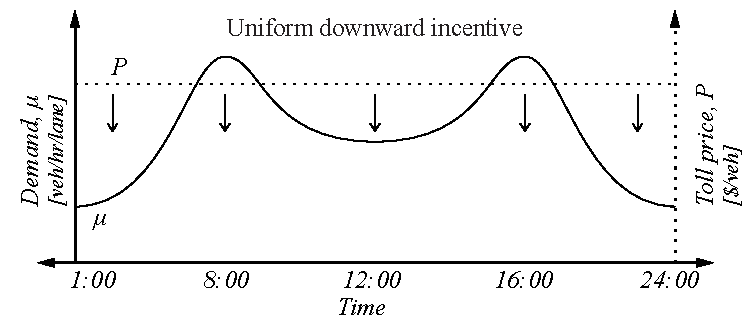
\includegraphics[width=\textwidth]{figures/flatprice}
	\centering
	\caption{Fixed toll pricing incentive}
	\label{fig:flatprice}
\end{subfigure}
\begin{subfigure}[h]{\linewidth}
	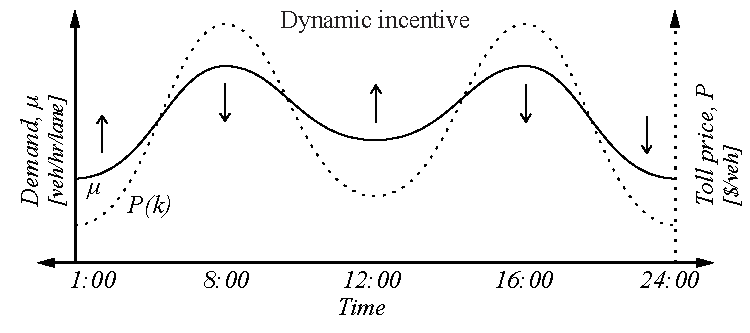
\includegraphics[width=\textwidth]{figures/dynamicprice}
	\centering
	\caption{Dynamic toll pricing incentive}
	\label{fig:dynamicprice}
\end{subfigure}
\label{fig:incentives}
\caption{Incentive effect on demand}
\end{figure}

The obvious solution to this problem is to dynamically adjust pricing based on demand to help discourage travel during congested periods and shift it to periods of low demand (see Figure~\ref{fig:dynamicprice}). Dynamic tolls have long been proposed as a solution to provide a more targeted congestion mitigating incentive, as has been done for decades in other non-automobile transportation sectors (e.g., bus, rail, and air travel), but have seldom been implemented due to negative political appeal [CITE]. Travelers generally do not want to pay for travel, let alone be subject to increased costs that they perceive as having little control over. Moreover, without any feasible alternative travel options, dynamic road pricing is little more than extortion. 

An alternative approach that has been proposed is the concept of travel credits [CITE], exploiting the aspect of finite roadway capacity as the basis for a ``cap and trade'' type model for mitigating congestion by crediting travelers for not traveling during the peak. Another more market based evolution of the approach has also been proposed, enabling travelers to ``sell'' their trip rights to the highest bidder, achieving a similar goal without the need for governments to credit travelers. Recently a great deal of hype has been drawn around the concept of Mobility as a Service (MaaS) where ``travel brokers'' like automated travel agencies provide integrated multi-modal trip packages to users for travelers. However, few of these concepts other than dynamic pricing have had little traction outside of academia in recent years, but some technology companies have implemented conceptually similar trip routing and payment integration features in their platforms (e.g., mobile payment systems with transit and ride hailing services), laying the groundwork for such concepts. 

The proposed mechanism is not necessarily a new concept, nor is it a radical technologically driven revolution, but merely an attempt to implement efficient congestion reducing market mechanisms by augmenting existing conventional revenue collection technologies (e.g., automated tolls). The proposed concept is simple, travelers have the option to purchase trips ahead of time while the price remains low, or at some fixed discount rate, with the option to sell unused trips back to the system at market rate. The proposed mechanism is intended to provide the following transportation operational benefits:
\begin{description}
	\item[Reduce congestion] with targeted demand responsive pricing, discouraging travel during congested periods without dampening economic activity during low demand times.
	
	\item[Encourage travel planning] not only through pricing, but provides travelers with information about expected demand based on booked trips.
	
	\item[Discourage wasteful behavior] by letting users sell unused booked trips and avoiding ``use it or lose it'' behavior.
	
	\item[Provide realtime future demand] data as a result of the pre-booked trip payment log.
\end{description}


%------------------------------------------------

\section{Conceptual framework}
The basic concept for the system is shown in Figure~\ref{fig:systemmodel}, where travel demand (e.g., over a bridge, along a corridor, or in a zone) can be divided into discrete travel windows (e.g., between 8:00-9:00) where there is a finite number of capacity available (e.g., a road capacity of 2,000 vehicles per hour). Travelers then have the option to pre-purchase a planned trip from the available capacity, with price increasing as booked trips in that time-frame increase. This encourages travelers to purchase trips ahead of time while the price remains low or discounted as well as potentially avoid traveling during those peak periods as the price increases towards capacity. Otherwise, travelers that do not pre-purchase their trip are subject to the ``market rate'' price determined by some price function at the time of travel, as is done in conventional dynamic pricing.

\begin{figure}[h]
	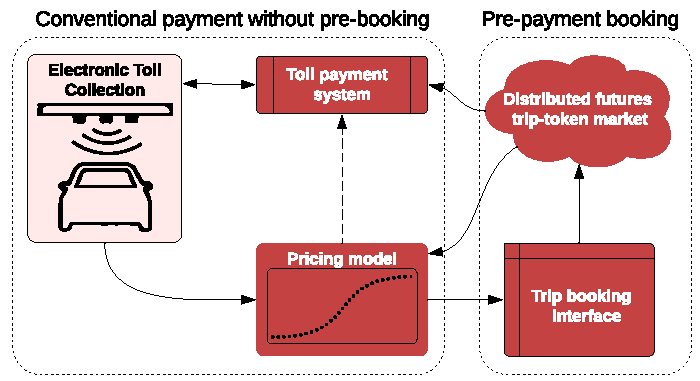
\includegraphics[width=\linewidth]{figures/systemmodel}
	\centering
	\caption{Conceptual system model}
	\label{fig:systemmodel}
\end{figure}

\subsection{Distributed market mechanism}
Just like in the past where tolls were once paid using physical tokens, this modern 21\textsuperscript{st} century version uses digital crypto-currency tokens instead. Unlike old tokens, which could be used at any time and only benefits were to avoid carrying exact change and sometimes a slight discount in bulk, crypto-tokens can fluctuate in price and contain secure encrypted data regarding who owns it and when it can be used. Time (i.e., travel arrival times) is broken down into arbitrarily small quantum units of time, such as 1, 5, or 15 minute intervals, for every time increment until some distance future time horizon (e.g., from now until one year). The increment depends on the desired resolution of the system and any computational limitations associated. 

Each time unit then becomes tokenized in a distributed crypto market. When travelers book their desired time window, they effectively purchase a sequential bundle of tokens. For example, a time window from 8am to 9am will have 60 tokens of 1 minute. The tokens will also contain data linking the individual time increment to all others associated with the larger time window. The price of that window then depends upon the sum of token prices across that range. The prices will then fluctuate based on the pricing function, which depends upon the number of travelers that have purchased the same overlapping tokens.

There are two benefits to having users purchase small tokenized units of time, rather than fixed large chunks of time (e.g., where users can only buy between 8am-9am, not 8:15am-8:45am). First is that it offers users greater flexibility in deciding when and how narrow their travel window will be. Second it further encourages users be punctual and to shift their travel times away from congested periods. For example, 8:00am to 9:00am are congested and thus expensive, but users can still achieve a discount by shifting from 7:30am to 8:30am, which only overlaps halfway with the congested times.

\subsection{Booking interface}
A basic booking interface could be a website or app where users can purchase their trip by time slot for a given date period (e.g., hourly time slots for a given date). For convenience, it would be wise to provide the option to buy trips in bulk for commuters (e.g., 9am-10am and 5pm-6pm time slots every Monday-Friday for the next month), as well as a customizable option for irregular trips. The system can then be easily integrated with existing toll collection and payment systems.

\subsection{Pricing}
Although pricing could be determined by some free floating free market price as long as it is calibrated to match the limited ``supply'' of road capacity, such an uncontrollable system may be unstable and result in public dissatisfaction. Alternatively, an engineered market price could be determined using a parametric function designed to achieve the best possible results while remaining stable. An example pricing function shown in Figure~\ref{fig:costflow} uses an S-shaped sigmoid as a function of traffic density $k$. 

\begin{figure}[h]
	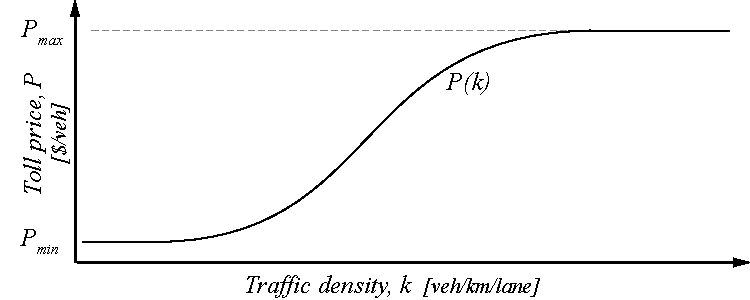
\includegraphics[width=\linewidth]{figures/costdensity}
	\centering
	\caption{Pricing sigmoid function}
	\label{fig:costflow}
\end{figure}

\noindent Unlike a monotonic function that could increase cost to infinity or decrease to zero, a sigmoid allows for price minimum $P_{min}$ and maximum $P_{max}$ boundaries to be set, while remaining as a conveniently smooth continuous function that can be expressed as

\begin{equation}
P(k) = P_{min} + \frac{P_{max} - P_{min}}{1 + e^{\alpha - \beta k}}
\label{eq:price}
\end{equation}

\noindent where $\alpha$ and $\beta$ are tuning parameters to specify the horizontal shift and ``steepness'' of the function, respectively. 

A potentially useful feature of using a bounded sigmoid is that it can be presented to the public as a discount feautre for pre-booked and off-peak travelers, not a surcharge (e.g., pre-booked off-peak for 50\% off full toll price, rather than presented as 50\% higher than regular toll price), helping to make it politically more palatable. Of course, the upper boundary will need to be set high enough to collect sufficient net revenue.

\subsection{Traffic flow}
\begin{figure*}[ht!]
	\hfill
	\centering
	\begin{subfigure}[h]{0.25\linewidth}
		\centering
		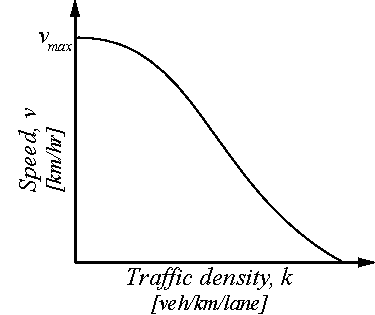
\includegraphics[width=\textwidth]{figures/speeddensity}
		\caption{Speed-density}
		\label{fig:speeddensity}
	\end{subfigure}
	\hfill
	\begin{subfigure}[h]{0.25\linewidth}
		\centering
		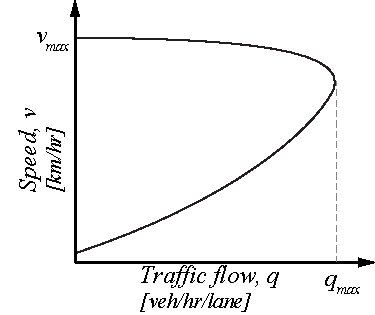
\includegraphics[width=\textwidth]{figures/speedflow}
		\caption{Speed-flow}
		\label{fig:speedflow}
	\end{subfigure}
	\hfill
	\begin{subfigure}[h]{0.25\linewidth}
		\centering
		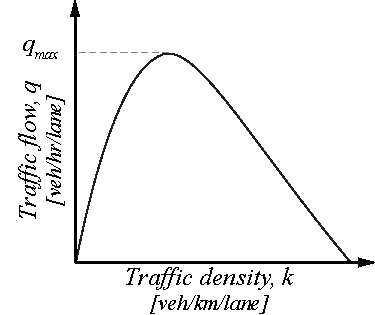
\includegraphics[width=\textwidth]{figures/flowdensity}
		\caption{Flow-density}
		\label{fig:flowdensity}
	\end{subfigure}
	\hfill
	\caption{Macroscopic Fundamental Diagram}
	\label{fig:MFD}
\end{figure*}

Although the dynamic pricing could be based on traffic speed, simply increasing when speed decreases by some function, the pricing function in this case is based on traffic density. This is for two reasons, first is that it enables the pricing function to be integrated with the futures market, which is based on some expected trip density. Second, if the goal is to increase infrastructure utilization and efficiency, not simply maintain high speeds, then speed is not a reliable measure of demand because traffic speed will remain relatively stable before smooth flow breaks down. This can be explained by the classical macroscopic fundamental diagram (MFD) in Figure~\ref{fig:MFD} where traffic speed and flow are inextricably linked by density. Figures~\ref{fig:speedflow} and ~\ref{fig:speeddensity} show that speed is relatively stable until some critical traffic density in Figure~\ref{fig:flowdensity} causes smooth traffic flow to break down at $q_{max}$.



\subsection{Smoothing expected travel density}
Although a flexible travel time window can be specified (e.g., 8:12 $\pm$ 30 mins), in practice it is likely that users will simply pick rounded numbers (e.g. 8:00), resulting in unrealistically concentrated trip densities that will vary in actual arrival time. Converting from pre-booked trips and into expected travel density can be achieved by smoothing the finite trips using a Kernal Density Estimation (KDE) 

\begin{equation}
\hat{k}(t) = \frac{1}{n} K_h (t - t_i) = \frac{1}{nh} \sum\limits_{i=1}^n K \frac{t-t_i}{h}
\label{eq:kde}
\end{equation}

\noindent where $\hat{k}(t)$ is the estimated density function for time $t$, $K$ is the non-negative kernel function (e.g., Gaussian normal curve), and $h$ is a smoothing bandwidth parameter that must be greater than 0. KDE essentially functions by cumulatively applying a continuous density function $K$ at each finite sample point, providing a smoothed probability distribution, such as shown in Figure~\ref{fig:kernal}. 

\begin{figure}[h]
	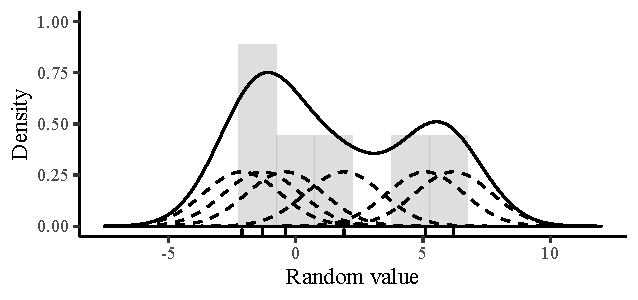
\includegraphics[width=\linewidth]{figures/KDE.pdf}
	\centering
	\caption{Kernel Density Estimation using Gaussian function}
	\label{fig:kernal}
\end{figure}

Once a smooth and stable value of future traffic density $\hat{k}(t)$ is calculated in Equation~\eqref{eq:kde}, it can be easily inputted into the pricing function in Equation~\eqref{eq:price} to obtain an estimated future toll price at that travel window. This process is continually updated until the horizon of the trip time window is reach. At this point the sale of future trips in the ``futures market'' is closed to pre-booking and any travel must be paid at the conventional real time market price based on the actual observed traffic density.

It is possible, and likely, that there will be discrepancy between the futures price and the real time market price, just as is the case in financial futures markets. There are two possible outcome scenarios for this. First is if the futures rate is lower than the market rate (dynamic or otherwise). This is because too few people pre-booked their trips, yielding a large discount against the conventional toll for the pre-booked travelers, thus incentivizing more people to adopt pre-booking. The possible downside is there will be limited congestion mitigation effects until sufficient market penetration is reached. The second case is if the futures rate is higher the market rate. This would occur if too many travelers failed to meet their target window or didn't show up at all, and did not sell their travel tokens. The travelers would incur a loss on their token, either partially if sold or in full if not sold; thus incentivizing travelers to be punctual. 

\section{Safeguards and practical constraints}
When creating a new market, care must be taken to ensure operation is smooth and stable. The following subsections discuss several basic market constraint recommendations.

\subsection{Market manipulators and exploitation}
When profit is to be made by selling unused trips, there will be those that seek to maximize profit by exploiting the system.  Thus to prevent users from inappropriately exploiting the system, restrictions should be set. For example, to prevent users from manipulating the market price, a practical restriction could limit users to only purchasing one trip per time slot (otherwise it would be a travel impossibility), or to limit the number of sales a user can make to ensure a net profit cannot be made. Ensuring zero profit would also help avoid any user tax complexities. Although restrictions may seem market prohibitive, the intent of the system to promote efficient travel and revenue collection, not market capitalization. 

\subsection{Price limits}
To avoid reaching outrageous prices and the public backlash that follows [cite Virginia example and uber surge pricing], reasonable upper limits on price should be set to avoid public backlash. Similarly, a lower price limit could also be set to provide a baseline revenue collection and travel disincentive.

\subsection{Pricing calibration}
The pricing function will need to be calibrated to match demand sensitivity as well as meet revenue obligations, while remaining politically palatable. Ideally the upper bound will be kept as low as possible to avoid public dissatisfaction, but high enough to achieve the desired shift in travel behavior. The lower bound must also be kept low enough to encourage a shift in travel behavior, but high enough to collect sufficient revenue. Research will be needed to measure user arrival time demand elasticity, that is how sensitive are travelers to increases in price. From this, the function can be optimized to balance operations with revenue, and will likely need regular tuning to adjust for current conditions. 

\subsection{Time scale}
Although theoretically possible to operate with narrow time intervals, such as $<$1-second, the computational limitations of accounting for that many tokens and transferring every second is likely intractable. Moreover, travelers probably will not bother with such detail nor be held to such precision. It's likely that users will pick a target time $\pm$ some buffer time (e.g., $\pm$ 30 minutes from expected arrival). However, it is uncertain whether travelers will be equally as likely to arrive early as late, which can be modeled with a Guassian normal curve; or perhaps travelers trend on being late but not early, which can be modeled with a log-normal curve. Research is needed in this area to determine feasible parameters and the relative reliability of travelers. Alternatively, the system could be designed in such a way to allow for users to specify their desired travel window, offering greater discount to more punctual travelers and a penalty to those that fail to meet their target.

\section{Toy example}
 As an example application, suppose there are two adjacent cities as shown in Figure~\ref{fig:toymap}, which are separated by a body of water. The two cities are connected by a six lane bridge, three lanes in each direction, that carries 100,000 trips per day with an existing fixed toll of \$7.75.
 
 \begin{figure}[h]
 	\centering
 	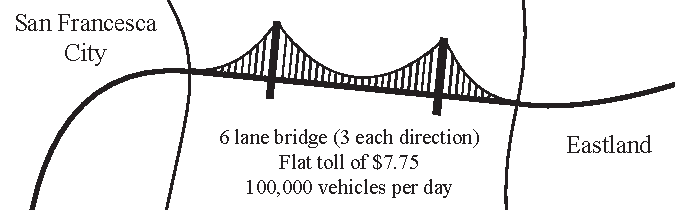
\includegraphics[width=\linewidth]{figures/silvergate}
 	\caption{Toy example scenario}
 	\label{fig:toymap}
 \end{figure}
 
 \noindent For simplicity, assume the traffic flow is balanced in each direction but possess a demand distribution with two peaks as shown in Figure~\ref{fig:toydem}. Note that the demand in Figure~\ref{fig:toydem} shows demand as traffic density, not volume. For reference, optimal traffic flow is $\approx 20 \sfrac{veh}{km}$ and traffic flow begins to become unstable above $\approx 30 \sfrac{veh}{km}$.
   
 \begin{figure}[h]
     \begin{subfigure}[h]{\linewidth}
     	\centering
     	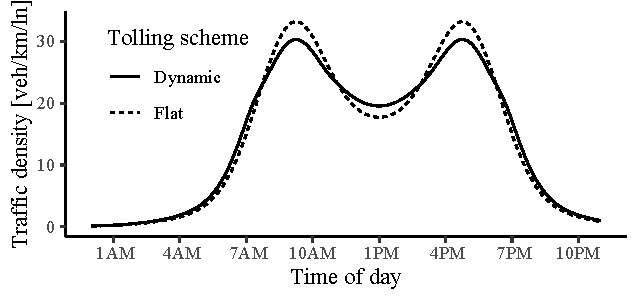
\includegraphics[width=\textwidth]{figures/toydemand}
     	\caption{Demand density}
     	\label{fig:toydem}
     \end{subfigure}
     \begin{subfigure}[h]{\linewidth}
     	\centering
     	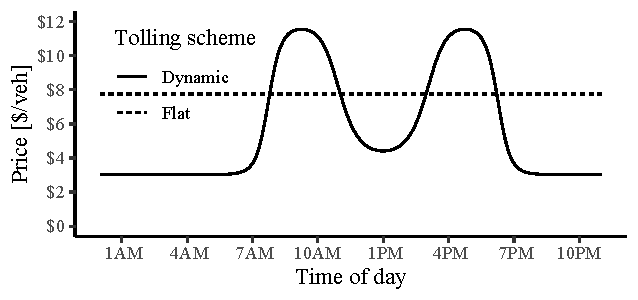
\includegraphics[width=\textwidth]{figures/toytoll}
     	\caption{Toll pricing}
     	\label{fig:toytoll}
     \end{subfigure}
     \caption{Toy example toll pricing and demand density}
     \label{fig:toymodel}
 \end{figure}
 
 There are two demand distributions, one distribution results from a flat toll which is constructed from the sum of four Gaussian functions characterized by means at 9:00, 12:00, 14:00 and 17:00, each with a standard deviation of 2. The other distribution is a result of demand shift incentivized by the dynamic toll price in Figure~\ref{fig:toytoll}, which was calculated using the sigmoid function in Figure~\ref{fig:toyprice}.
 
 \begin{figure}[h]
 	\centering
 	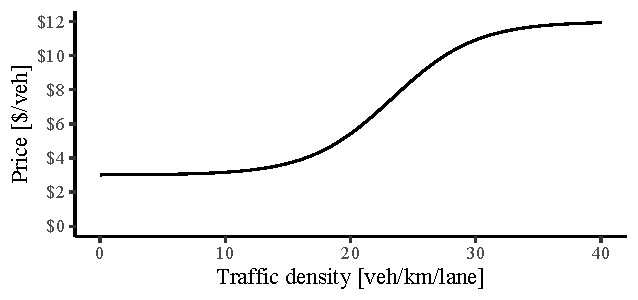
\includegraphics[width=\linewidth]{figures/toyprice}
 	\caption{Toy pricing sigmoid function}
 	\label{fig:toyprice}
 \end{figure}
 
 
 The sigmoid function uses the parameters in Table~\ref{tab:toyprice} with values for Equation~\eqref{eq:price} set arbitrarily to have a base $P_{min}$ lower and a $P_{max}$ higher than the fixed toll.  
 
  \begin{table}[h]
 	\centering
 	\caption{Toy example pricing parameters}
 	\begin{tabular}{ c c l}
 		\toprule
 		Parameter   & Value  & Description                          \\ \hline
 		$P_{fixed}$ & \$7.75 & \small Fixed toll price                     \\
 		$P_{min}$   & \$3    & \small Minimum dynamic toll price           \\
 		$P_{max}$   & \$12   & \small Maximum dynamic toll price			\\
 		$\alpha$    & 7      & \small Price calibration parameter \\
 		$\beta$     & 0.3    & \small Price calibration parameter \\
 		$E$         & 0.4    & \small Elasticity \\ \bottomrule
 	\end{tabular}
 	\label{tab:toyprice}
 \end{table}

The approximated demand resulting from dynamic pricing are calculated using simple micro-economic principles of elasticity. For this, a typical isoelastic demand function of
  \begin{equation}
 \Delta\mu = e^{-E \cdot \Delta P} - 1
 \end{equation} 
 was used with a fairly inelastic elasticity $E$, of 0.4 and centered on zero, as shown in Figure~\ref{fig:toyelasticity}.
  
  \begin{figure}[h]
 	\centering
 	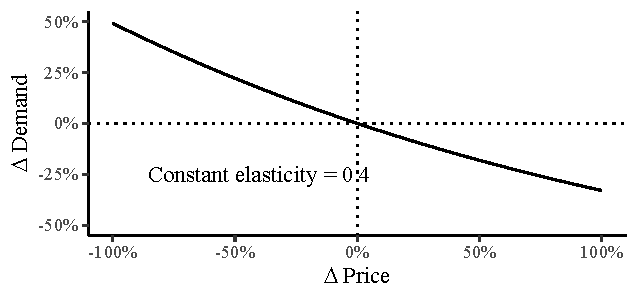
\includegraphics[width=\linewidth]{figures/toyelasticity}
 	\caption{Price elasticity}
 	\label{fig:toyelasticity}
 \end{figure}
 
  
The net revenue resulting from the simple example actually yielded a slight increase in revenue in this case, as shown in Figure~\ref{fig:toyrevenue}, despite offering a discounted $P_{min}$ toll.
 
 \begin{figure}[h]
 	\centering
 	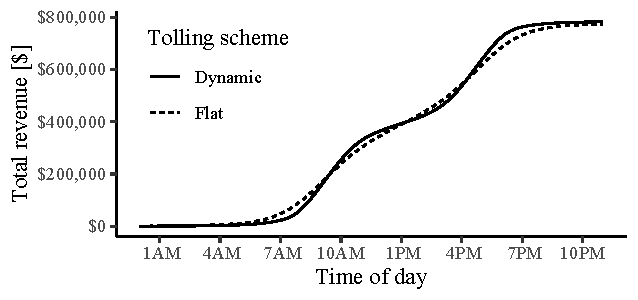
\includegraphics[width=\linewidth]{figures/toyrevenue}
 	\caption{Aggregate revenue}
 	\label{fig:toyrevenue}
 \end{figure}
 
This shows that a modest adjustment in price results in demand shift (i.e., commuters shifting behavior to avoid high tolls) without revenue loss. This is especially true if overall demand does not decrease as could be the case with introducing flat tolls. Of course, an increase in revenue is not guaranteed and depends upon the parameters selected in the pricing function. An obvious solution to this is to calibrate the parameters to optimize for revenue and/or congestion, or alternatively the pricing function itself could be altered to suit a particular scenario (e.g., use artificial intelligence to set prices to maximize an objective). The booking apparatus lends itself to this optimization, providing data of future demand to help best predict optimal prices; a feature unavailable in current dynamic pricing systems. Moreover, integration and revenue sharing policies with other modes, such as public transit, could yield a more globally optimal solution. 

\section{Future futures}
Although presented for a simple bridge toll, it can be easily expanded to other applications, such as corridor tolls, congestion pricing zones, transit fares, ride hailing, or applications beyond transportation. This could provide a basic framework for a broader more mode agnostic transportation system, which is of growing importance as ride sharing, hailing, and other future mobility platforms emerge, 

\section{Tech to market plan}
There are essentially three basic implementations of a futures market:
\begin{description}
    \item[An existing dynamic toll system] can be easily augmented with a futures market to further improve demand optimization with only software changes necessary. In this case, the futures market would have no negative impact revenue collection. 
    
    \item[A fixed toll system] can use a futures market to introduce dynamic pricing as an ``opt in'' program, incentivizing users with discounts for pre-booking travel during periods of low demand. Infrastructure investment would be minimal, especially if electronic tolling is already in place. A futures market in this case would be a soft way to introduce dynamic pricing in an otherwise politically hostile environment. In this case the futures market may impact revenue collection if the fixed toll is not sufficiently high enough. Since it is impossible/unreasonable for the futures price to exceed the fixed price, thus the fixed fare becomes $P_{max}$ and care must be taken to ensure it is set sufficiently high enough to achieve desired revenue. However, it may be possible that with improved traffic flow there may be a net revenue benefit in collection that would have otherwise been reduced at jam density.
    
    \item[No existing toll system] is naturally the most difficult case to implement, requiring both hardware and software investment, as well as inevitable political backlash from any tolling introduced.
\end{description}


\subsection{Things to build}
\begin{itemize}
    \item User interface\\
    \$X for N front-end developers [Jon \& John]?
    
    \item Decentralized market\\
    \$X for N developers crypto developers [Charlie?]
    
    \item Integration with existing payment system\\
    \$X for N developers crypto developers [Jon, John, \& Charlie?]
    
    \item Data storage system for calibration and prediction.\\
    \$X for N developers crypto developers [Nick, Jon, John, \& Charlie?]
    
    \item Pricing model integration with real-time traffic data
    \$X for N developers crypto developers [Nick?]
\end{itemize}

\subsection{Funding bits}
\begin{itemize}
    \item Startup seed for above development\\
    \$X total seed
    \item Transaction fee for ongoing maintenance and development\\
    $\%1 \times \$775,000=\$7,750/day$
\end{itemize}


\subsection{Barriers to entry}
\begin{itemize}
    \item Existing toll policies and the refusal to change, or the lack thereof
\end{itemize}

%----------------------------------------------------------------------------------------
%	BIBLIOGRAPHY
%----------------------------------------------------------------------------------------

\printbibliography[title={Bibliography}] % Print the bibliography, section title in curly brackets

%----------------------------------------------------------------------------------------

\end{document}
